\section{Training Pipeline}

\subsection{Data Preprocessing}

\subsubsection{Converting the Data from CSV to Parquet}

The data is stored in CSV format. The Parquet format is a binary columnar storage format that is more efficient than CSV for reading and writing data. The training data consists of 42,299,771 rows, while the testing data consists of 42,999,775 rows.

\subsubsection{Data Cleaning}

To clean the data, we drop the rows where more than 5 null features. This helps us remove any incomplete or missing data. After performing this operation, the training data consists of 33,088,764 rows, while the testing data consists of 33,678,677 rows.


\subsubsection{Data Resplitting}

To balance the training and testing data, we move 60\% of the testing data to the training data. This results in the training data consisting of 53,299,746 rows, while the testing data consists of 13,467,695 rows. The ratio of the training data to the testing data is 75:25.

\subsubsection{Add Timestamps to the Data}

After extracting the unique users and items, we add timestamps to the data. The timestamps are added to the training and testing data to help us track the time each user interacted with an item.

The following table shows the changes made to the data during the preprocessing phase:

\begin{table}[ht]
\centering
\begin{tabular}{|c|c|c|c|}
\hline
\textbf{Data Set} & \textbf{Original Rows} & \textbf{Data After Cleaning} & \textbf{Data After Resplitting} \\
\hline
Training Data & 42,299,771 & 33,088,764 & 53,299,746 \\
\hline
Testing Data & 42,999,775 & 33,678,677 & 13,467,695 \\
\hline
\end{tabular}
\caption{Data Reprocessing}
\label{tab:data-reprocessing}
\end{table}


\subsection{Retrieval Model Training}

The retrieval model is trained using the training data. The model is trained using the following hyperparameters:

\begin{itemize}
\item Batch Size: 28672
\item Number of Epochs: 20
\item Optimizer: Adam
\item Loss Function: Categorical Crossentropy
\item Model: DLRM
\end{itemize}


The results of shows that the training loss decreases as the number of epochs increases. and the Recall of the model increases as the number of epochs increases. The model achieves a recall of 0.3 after 20 epochs as shown in Figure \ref{fig:RetrievalModelTraining}.

\begin{figure}[H]
    \centering
    \begin{subfigure}{.5\textwidth}
        \centering
        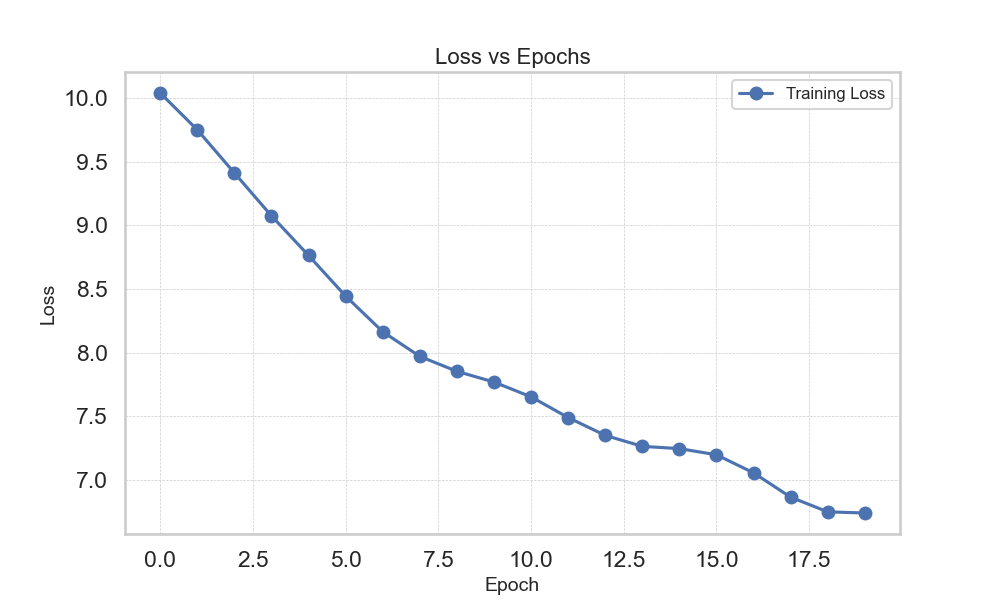
\includegraphics[width=0.95\linewidth]{assets/training_loss.png}
        \caption[Retrieval Model Loss]{Retrieval Model Loss}
        \label{fig:RetrievalModelLoss}
    \end{subfigure}%
    \begin{subfigure}{.5\textwidth}
        \centering
        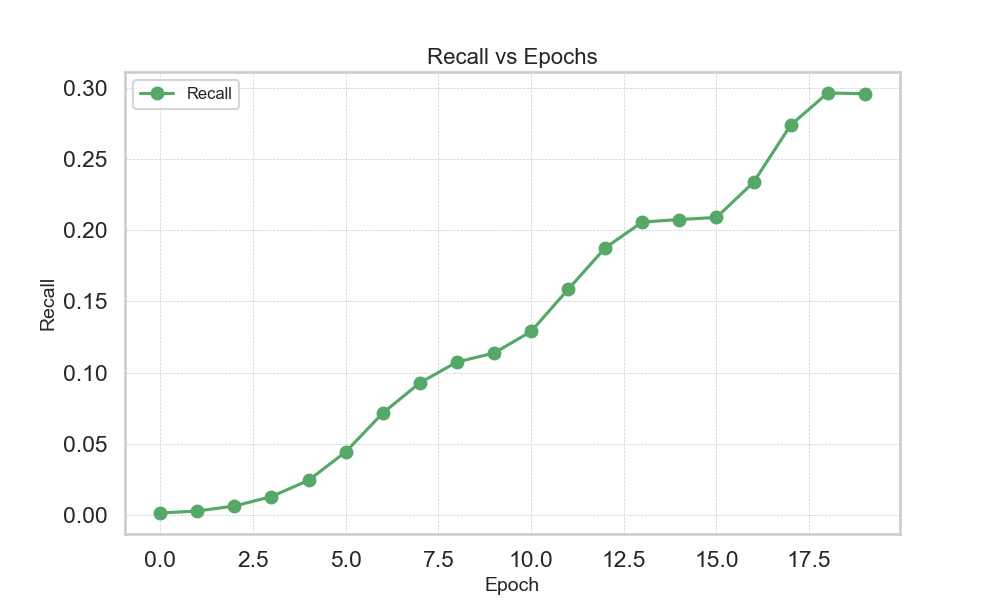
\includegraphics[width=0.95\linewidth]{assets/recall_epochs.png}
        \caption[Retrieval Model Recall]{Retrieval Model Recall}
        \label{fig:RetrievalModelRecall}
    \end{subfigure}
    \caption[Retrieval Model Training]{Retrieval Model Training}
    \label{fig:RetrievalModelTraining}
\end{figure}


\subsection{Generate Item Embeddings}

The item embeddings are generated using the trained retrieval model.

\subsection{Ranking Model Training}

The ranking model is trained using the training data. The model is trained using the following hyperparameters:

\begin{itemize}
\item Batch Size: 204800
\item Number of Epochs: 2
\item Optimizer: Adam
\end{itemize}

The results show that the model achieves a AUC of 0.67 after 2 epochs and a recall of 0.34
